\documentclass[12pt,a4paper]{report}

\usepackage[utf8]{inputenc}
\usepackage[T1]{fontenc}
\usepackage[english]{babel}
\usepackage[top=1cm,bottom=2cm,left=1cm,right=1cm]{geometry}
%\usepackage{url}
%\usepackage{fancyhdr}
\usepackage{sectsty}
\usepackage{wrapfig}
\usepackage{titlesec}
\usepackage{setspace}
\usepackage{graphicx}
\usepackage{lmodern}
\usepackage{url}
\usepackage{amsmath}
\usepackage{amssymb}
\usepackage{mathrsfs}
\usepackage{fancyhdr}
\usepackage{gensymb}
\usepackage{enumerate}
\usepackage{caption}
\usepackage{hyperref} % Créer des liens et des signets 
\usepackage[cc]{titlepic}
\usepackage{listing}

\title{
\rule{15cm}{1pt} \\
\Large {\bfseries Machine Learning} \\
\Large {\bfseries Assignement 13 GoogleNet vs ResNet}\\
\rule{15cm}{1pt}}
\author{Sami Sellami}

\titlepic{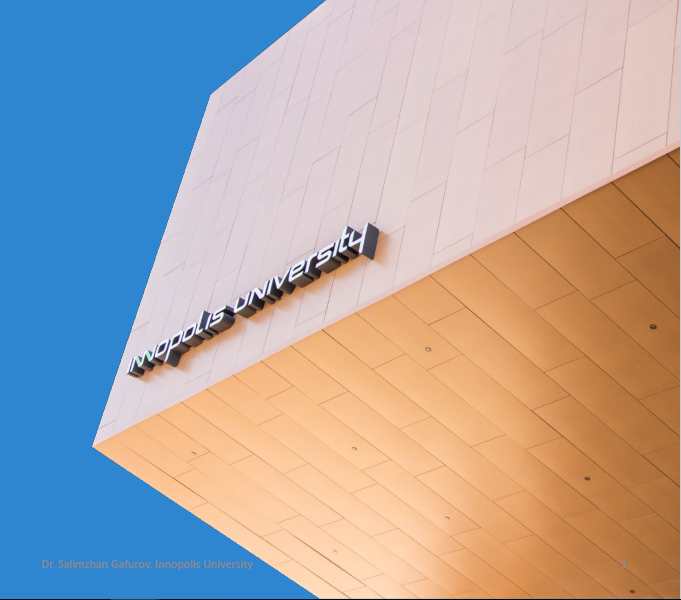
\includegraphics[width=15cm]{Innopolis_image.png}} 
\date{\today}

\begin{document}
\pagenumbering{arabic}
\setcounter{page}{1}
\setcounter{secnumdepth}{1}
	
\fontfamily{ptm}\selectfont

\maketitle

\titlelabel{\thetitle)\quad}
\titlespacing{\chapter}{0cm}{0cm}{0cm}
\titlespacing{\section}{0.2cm}{0cm}{0cm}


\begin{enumerate}
\item \textbf{Introduction}:

    A Convolutional Neural Network (CNN, or ConvNet) is a multi-layer neural networks designed to recognize visual patterns directly from pixel images with minimal preprocessing. The ImageNet project is a large visual database designed for use in visual object recognition software research. The ImageNet project runs an annual software contest, the ImageNet Large Scale Visual Recognition Challenge (ILSVRC), where software programs compete to correctly classify and detect objects and scenes. The most famous competitors who achieved a very substantial improvement in the classification error are GoogleNet and ResNet who were the first competitors able to compete with the human level performance in recognizing the images, in this paper, we propose to make a comparison of the two networks showing the key contributions, differences and results of the two architectures 
\end{enumerate} 

\begin{enumerate}

\item \textbf{GoogleNet}:

This is the winner of the 2014 competition, it achieved a  top-5 error rate of 6.67\%, the network used a CNN inspired by LeNet (the 1998 winner of the competition) their architecture consisted of 22 layers deep CNN but reduced the number of parameters from 60 millions to 4 millions

\textbf{Key contribution:} \\
The paper showed that increasing the size of the network does not mean necessarily improving the performance of the neural network, as a matter of fact bigger size means larger number of parameters and thus more risk of overfitting, moreover larger networks implies an increase use of computational resources, the ideas that propose the paper for solving those problems is to move from fully connected to sparsely connected architectures.  

\textbf{Architecture details:}\\
GoogleNet is based on layer-by-layer construction in which one should analyze the correlation statistics of the last layer and cluster them into groups of units with high correlation, these clusters form the units to the next layers and are connected to the units of the next layer, they also proposed to add an alternative parallel pooling path in each such stage, another idea that the team proposed is to apply dimensions reductions and projections wherever the computational requirement would increase too much  
 
\begin{center}
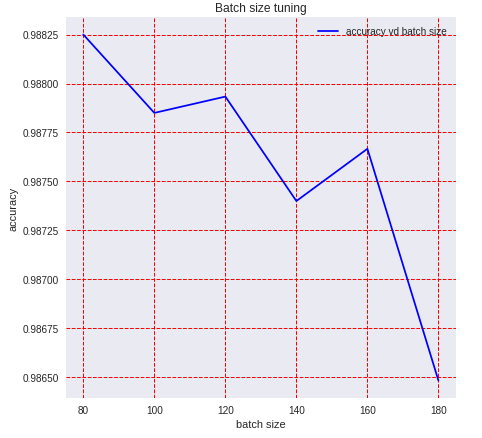
\includegraphics[width=15cm]{Capture1.png}
%\captionof{figure}{Accuracy as a function of number of units in CNN with two layer}
\end{center}

In general , an inception network is a network consisting of modules of the above type stacked upon each other 
the benefits of this architecture is that it allows increasing the number of units at each stage significantly without an uncontrolled blow up in computational complexity 	

\textbf{Key results}\\
The final submission of the team obtained an top 5 error of $6.67\%$ on both the validation and testing data, this was a 56.5\% relative reduction compared to the SuperVision approach in 2012, and about 40 relative reduction compared to the previous year’s best approach (Clarifai), both of which used external data for training the classifiers. \\

\item \textbf{ResNet:}\\
ResNet which stands for residual neural network is the winner of the 2015 competition introduced a new architecture with skip connection and feature heavy batch normalization, thanks to this technique the team was able to train a neural network with 152 layers and achieving a top 5 rate of 3.57\% which beats human-level performance on this dataset

\textbf{Key contribution:} 
The paper faced the problem of vanishing gradient which hamper convergence from the beginning when we stack more layers in the network, to solve the problem they introduced a deep residual learning framework, Instead of hoping each few stacked layers directly fit a desired underlying mapping, they  explicitly let these layers fit a residual mapping. $F(x)= H(x)-x $. The original mapping is recast into $F(x)+x$. it is easier to optimize the residual mapping than to optimize the original one. 

\textbf{Architecture details:}
In their work the team have tested various plain/residual networks, plain networks are inspired by the VGG nets, the convolutional layers have $3\times 3$ filters and follow two simple rules; the layers have the same number of filters and if the feature maps halved the number of filter is doubled so as to preserve the time complexity per layer, they performed downsampling directly by convolutional layer that have stride 2 and the network ends by global average pooling layer and an 1000 way fully connected layer with softmax. 
Residual network on the other hand is based on plain network but with shortcut connections 

\begin{center}
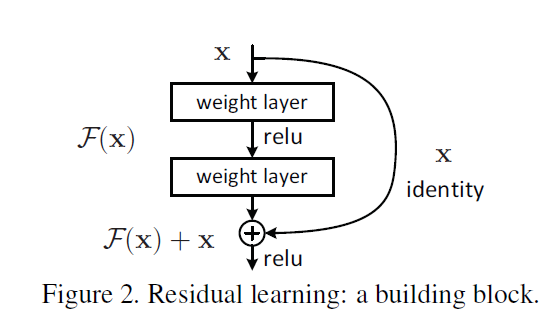
\includegraphics[width=7cm]{Capture2.png}
%\captionof{figure}{Accuracy as a function of number of units in CNN with two layer}
\end{center}

\textbf{Key results:}\\
Plain 	network: they evaluated 18 and 34 layers plain net, the results showed that the 34-layer plain net has higher validation error than the 18-layer plain net\\
Residual networks: like the plain network they did the test with 18 and 34 layers residual nets, the base line is the same as the plain net except that they have added a shortcut connection to each of pair of the $3 \times 3$ filters, this time the situation is reversed and the 34-layers nets demonstrated better results than the 18-layers, moreover the 34-layers showed better training and validation error this means that the degradation problem is well adressed in this architecture and they managed to improve accuracy from increased depth, also the residual net decreased the top 1 error to 3.5 \\
With these results the team also constructed an 101 and 152 layers networks by using more 3 layers blocks, although the depth is significantly increased the 152 layers has better accuracy, in fact the accuracy is increased with the depth of the network because there is no degradation problem the benefits of depth are now witnessed for all evaluation metrics.

\item \textbf{comparing the two methods:}
The two architectures addressed the issue of increasing the size of the network architecture, the latter causes usually more time and computational  resources need, GoogleNet for this, proposed to reduce the number of parameters by moving from fully connected to sparsely connected architectures, while ResNet on the other hand introduced a deep residual framework learning framework and which resolve the problem of vanishing gradient, the two architectures gave good results but ResNet was by far the best as it reached a top 5 rate of 3.57\%

\item \textbf{Conclusion:}\\
In the present report we did a concise study of two CNN architectures that won the ImageNet competition for image classification, namely GoogleNet and ResNet, the networks showed remarkable results during their respective years 2014 and 2015 and were able to compete with the human level performance, each method proposed a new approach for training the network, GoogleNet was based on layer-by-layer construction using sparsely connected layers while ResNet proposed a deep residual learning framework to resolve the problem of vanishing gradient allowing them to apply the famous 'we need to go deeper' internet meme in real situations.
  

 














\end{enumerate}
\end{document}	
